\documentclass{ximera}

%\usepackage{todonotes}

\newcommand{\todo}{}

\usepackage{esint} % for \oiint
\ifxake%%https://math.meta.stackexchange.com/questions/9973/how-do-you-render-a-closed-surface-double-integral
\renewcommand{\oiint}{{\large\bigcirc}\kern-1.56em\iint}
\fi


\graphicspath{
  {./}
  {ximeraTutorial/}
  {basicPhilosophy/}
  {functionsOfSeveralVariables/}
  {normalVectors/}
  {lagrangeMultipliers/}
  {vectorFields/}
  {greensTheorem/}
  {shapeOfThingsToCome/}
  {dotProducts/}
  {partialDerivativesAndTheGradientVector/}
  {../productAndQuotientRules/exercises/}
  {../normalVectors/exercisesParametricPlots/}
  {../continuityOfFunctionsOfSeveralVariables/exercises/}
  {../partialDerivativesAndTheGradientVector/exercises/}
  {../directionalDerivativeAndChainRule/exercises/}
  {../commonCoordinates/exercisesCylindricalCoordinates/}
  {../commonCoordinates/exercisesSphericalCoordinates/}
  {../greensTheorem/exercisesCurlAndLineIntegrals/}
  {../greensTheorem/exercisesDivergenceAndLineIntegrals/}
  {../shapeOfThingsToCome/exercisesDivergenceTheorem/}
  {../greensTheorem/}
  {../shapeOfThingsToCome/}
  {../separableDifferentialEquations/exercises/}
  {vectorFields/}
}

\newcommand{\mooculus}{\textsf{\textbf{MOOC}\textnormal{\textsf{ULUS}}}}

\usepackage{tkz-euclide}
\usepackage{tikz}
\usepackage{tikz-cd}
\usetikzlibrary{arrows}
\tikzset{>=stealth,commutative diagrams/.cd,
  arrow style=tikz,diagrams={>=stealth}} %% cool arrow head
\tikzset{shorten <>/.style={ shorten >=#1, shorten <=#1 } } %% allows shorter vectors

\usetikzlibrary{backgrounds} %% for boxes around graphs
\usetikzlibrary{shapes,positioning}  %% Clouds and stars
\usetikzlibrary{matrix} %% for matrix
\usepgfplotslibrary{polar} %% for polar plots
\usepgfplotslibrary{fillbetween} %% to shade area between curves in TikZ
%\usetkzobj{all}
\usepackage[makeroom]{cancel} %% for strike outs
%\usepackage{mathtools} %% for pretty underbrace % Breaks Ximera
%\usepackage{multicol}
\usepackage{pgffor} %% required for integral for loops



%% http://tex.stackexchange.com/questions/66490/drawing-a-tikz-arc-specifying-the-center
%% Draws beach ball
\tikzset{pics/carc/.style args={#1:#2:#3}{code={\draw[pic actions] (#1:#3) arc(#1:#2:#3);}}}



\usepackage{array}
\setlength{\extrarowheight}{+.1cm}
\newdimen\digitwidth
\settowidth\digitwidth{9}
\def\divrule#1#2{
\noalign{\moveright#1\digitwidth
\vbox{\hrule width#2\digitwidth}}}




% \newcommand{\RR}{\mathbb R}
% \newcommand{\R}{\mathbb R}
% \newcommand{\N}{\mathbb N}
% \newcommand{\Z}{\mathbb Z}

\newcommand{\sagemath}{\textsf{SageMath}}


%\renewcommand{\d}{\,d\!}
%\renewcommand{\d}{\mathop{}\!d}
%\newcommand{\dd}[2][]{\frac{\d #1}{\d #2}}
%\newcommand{\pp}[2][]{\frac{\partial #1}{\partial #2}}
% \renewcommand{\l}{\ell}
%\newcommand{\ddx}{\frac{d}{\d x}}

% \newcommand{\zeroOverZero}{\ensuremath{\boldsymbol{\tfrac{0}{0}}}}
%\newcommand{\inftyOverInfty}{\ensuremath{\boldsymbol{\tfrac{\infty}{\infty}}}}
%\newcommand{\zeroOverInfty}{\ensuremath{\boldsymbol{\tfrac{0}{\infty}}}}
%\newcommand{\zeroTimesInfty}{\ensuremath{\small\boldsymbol{0\cdot \infty}}}
%\newcommand{\inftyMinusInfty}{\ensuremath{\small\boldsymbol{\infty - \infty}}}
%\newcommand{\oneToInfty}{\ensuremath{\boldsymbol{1^\infty}}}
%\newcommand{\zeroToZero}{\ensuremath{\boldsymbol{0^0}}}
%\newcommand{\inftyToZero}{\ensuremath{\boldsymbol{\infty^0}}}



% \newcommand{\numOverZero}{\ensuremath{\boldsymbol{\tfrac{\#}{0}}}}
% \newcommand{\dfn}{\textbf}
% \newcommand{\unit}{\,\mathrm}
% \newcommand{\unit}{\mathop{}\!\mathrm}
% \newcommand{\eval}[1]{\bigg[ #1 \bigg]}
% \newcommand{\seq}[1]{\left( #1 \right)}
% \renewcommand{\epsilon}{\varepsilon}
% \renewcommand{\phi}{\varphi}


% \renewcommand{\iff}{\Leftrightarrow}

% \DeclareMathOperator{\arccot}{arccot}
% \DeclareMathOperator{\arcsec}{arcsec}
% \DeclareMathOperator{\arccsc}{arccsc}
% \DeclareMathOperator{\si}{Si}
% \DeclareMathOperator{\scal}{scal}
% \DeclareMathOperator{\sign}{sign}


%% \newcommand{\tightoverset}[2]{% for arrow vec
%%   \mathop{#2}\limits^{\vbox to -.5ex{\kern-0.75ex\hbox{$#1$}\vss}}}
% \newcommand{\arrowvec}[1]{{\overset{\rightharpoonup}{#1}}}
% \renewcommand{\vec}[1]{\arrowvec{\mathbf{#1}}}
% \renewcommand{\vec}[1]{{\overset{\boldsymbol{\rightharpoonup}}{\mathbf{#1}}}}

% \newcommand{\point}[1]{\left(#1\right)} %this allows \vector{ to be changed to \vector{ with a quick find and replace
% \newcommand{\pt}[1]{\mathbf{#1}} %this allows \vec{ to be changed to \vec{ with a quick find and replace
% \newcommand{\Lim}[2]{\lim_{\point{#1} \to \point{#2}}} %Bart, I changed this to point since I want to use it.  It runs through both of the exercise and exerciseE files in limits section, which is why it was in each document to start with.

% \DeclareMathOperator{\proj}{\mathbf{proj}}
% \newcommand{\veci}{{\boldsymbol{\hat{\imath}}}}
% \newcommand{\vecj}{{\boldsymbol{\hat{\jmath}}}}
% \newcommand{\veck}{{\boldsymbol{\hat{k}}}}
% \newcommand{\vecl}{\vec{\boldsymbol{\l}}}
% \newcommand{\uvec}[1]{\mathbf{\hat{#1}}}
% \newcommand{\utan}{\mathbf{\hat{t}}}
% \newcommand{\unormal}{\mathbf{\hat{n}}}
% \newcommand{\ubinormal}{\mathbf{\hat{b}}}

% \newcommand{\dotp}{\bullet}
% \newcommand{\cross}{\boldsymbol\times}
% \newcommand{\grad}{\boldsymbol\nabla}
% \newcommand{\divergence}{\grad\dotp}
% \newcommand{\curl}{\grad\cross}
%\DeclareMathOperator{\divergence}{divergence}
%\DeclareMathOperator{\curl}[1]{\grad\cross #1}
% \newcommand{\lto}{\mathop{\longrightarrow\,}\limits}

% \renewcommand{\bar}{\overline}

\colorlet{textColor}{black}
\colorlet{background}{white}
\colorlet{penColor}{blue!50!black} % Color of a curve in a plot
\colorlet{penColor2}{red!50!black}% Color of a curve in a plot
\colorlet{penColor3}{red!50!blue} % Color of a curve in a plot
\colorlet{penColor4}{green!50!black} % Color of a curve in a plot
\colorlet{penColor5}{orange!80!black} % Color of a curve in a plot
\colorlet{penColor6}{yellow!70!black} % Color of a curve in a plot
\colorlet{fill1}{penColor!20} % Color of fill in a plot
\colorlet{fill2}{penColor2!20} % Color of fill in a plot
\colorlet{fillp}{fill1} % Color of positive area
\colorlet{filln}{penColor2!20} % Color of negative area
\colorlet{fill3}{penColor3!20} % Fill
\colorlet{fill4}{penColor4!20} % Fill
\colorlet{fill5}{penColor5!20} % Fill
\colorlet{gridColor}{gray!50} % Color of grid in a plot

\newcommand{\surfaceColor}{violet}
\newcommand{\surfaceColorTwo}{redyellow}
\newcommand{\sliceColor}{greenyellow}




\pgfmathdeclarefunction{gauss}{2}{% gives gaussian
  \pgfmathparse{1/(#2*sqrt(2*pi))*exp(-((x-#1)^2)/(2*#2^2))}%
}


%%%%%%%%%%%%%
%% Vectors
%%%%%%%%%%%%%

%% Simple horiz vectors
\renewcommand{\vector}[1]{\left\langle #1\right\rangle}


%% %% Complex Horiz Vectors with angle brackets
%% \makeatletter
%% \renewcommand{\vector}[2][ , ]{\left\langle%
%%   \def\nextitem{\def\nextitem{#1}}%
%%   \@for \el:=#2\do{\nextitem\el}\right\rangle%
%% }
%% \makeatother

%% %% Vertical Vectors
%% \def\vector#1{\begin{bmatrix}\vecListA#1,,\end{bmatrix}}
%% \def\vecListA#1,{\if,#1,\else #1\cr \expandafter \vecListA \fi}

%%%%%%%%%%%%%
%% End of vectors
%%%%%%%%%%%%%

%\newcommand{\fullwidth}{}
%\newcommand{\normalwidth}{}



%% makes a snazzy t-chart for evaluating functions
%\newenvironment{tchart}{\rowcolors{2}{}{background!90!textColor}\array}{\endarray}

%%This is to help with formatting on future title pages.
\newenvironment{sectionOutcomes}{}{}



%% Flowchart stuff
%\tikzstyle{startstop} = [rectangle, rounded corners, minimum width=3cm, minimum height=1cm,text centered, draw=black]
%\tikzstyle{question} = [rectangle, minimum width=3cm, minimum height=1cm, text centered, draw=black]
%\tikzstyle{decision} = [trapezium, trapezium left angle=70, trapezium right angle=110, minimum width=3cm, minimum height=1cm, text centered, draw=black]
%\tikzstyle{question} = [rectangle, rounded corners, minimum width=3cm, minimum height=1cm,text centered, draw=black]
%\tikzstyle{process} = [rectangle, minimum width=3cm, minimum height=1cm, text centered, draw=black]
%\tikzstyle{decision} = [trapezium, trapezium left angle=70, trapezium right angle=110, minimum width=3cm, minimum height=1cm, text centered, draw=black]


\title{Describe Everything}

\begin{document}

\begin{abstract}
characteristics
\end{abstract}
\maketitle




Analyzing a function means explaining how you determined all of the function's features, characteristics, and trends. \\

It is communication for other people to understand. \\






$\blacktriangleright$ \textbf{\textcolor{red!10!blue!90!}{Domain}}   \\
First, any function analysis would discuss the domain.  Perhaps the domain is already stated with the function definition. Otherwise, the function might be described with a formula. Then, the natural or implied domain can be deduced.  If the function is defined via a graph, then the implied domain can be deduced visually. A function might be defined via a function equation relating it to another function.  In this case, the equation would help us figure out the induced domain.\\

If a formula is provided, then we might categorize the function and obtain information about the domain.  Otherwise, we could look for numbers that would cause problems with the formula.

If a graph is the only information presented, then there is an unavoidable bubble of inaccuracy to work within.  The nature of drawing, the tools used and the person drawing, make inaccuracy simply a part of graphing or decerning information from a graph.

Even with a formula, piecing the graph together would give helpful clues. 

We want exact values when we can get them.  Otherwise, we settle for approximations. But we want algebra first.  Then we settle.\\









$\blacktriangleright$ \textbf{\textcolor{red!10!blue!90!}{Zeros}} \\
Identify all zeros.  This will involve solving equations that you create from your knowledge of the elementary functions. If a graph is the only information available, then look for intercepts.\\



$\blacktriangleright$ \textbf{\textcolor{red!10!blue!90!}{Continuity}} \\
The domain, discontinuities, and singularities should begin establishing intervals of continuity.  The endpoints or isolation numbers may require additional scrutiny.  \\


Identify discontinuities and singularities through the category of the function or operations involved.  These will show up as breaks in the graph. Describe the function's behavior around discontinuities and singularities with limit notation.\\








$\blacktriangleright$ \textbf{\textcolor{red!10!blue!90!}{End-Behavior}} \\
Think in terms of very very very big positive and negative numbers.  How does the function settle down for large domain numbers?  Describe end-behavior with limit notation. \\

Horizontal asymptotes are clues to end-behavior. Use technology to help you visualize.\\






$\blacktriangleright$ \textbf{\textcolor{red!10!blue!90!}{Behavior}} \\

\textbf{Rate-of-Change:} Identify intervals where the function increases and decreases will help identify extreme values, which often occur at critical numbers.  If you have the derivative, then its sign can tell you about the behavior of the original function.\\



$\blacktriangleright$ \textbf{\textcolor{red!10!blue!90!}{Extreme Values}} \\

Generally speaking, obtaining exact values of local maximums and mimimums and their critical numbers is going to be difficult without Calculus.  However, we know a lot about these in special situations. \\

If you have the derivative, then you can get exact values for critical numbers, which can be found where the derivative is zero or undefined. \\













$\blacktriangleright$ \textbf{\textcolor{red!10!blue!90!}{Range}}   \\
Generally speaking, you need all of the above informaiton to determine the range of a function.  A graph can be very helpful. \\



\begin{center}
\textbf{\textcolor{red!70!black}{We want exact values when we can get them.}}

\textbf{\textcolor{red!70!black}{Otherwise, we settle for approximations.}}
\end{center}








\begin{example} Complete Anlaysis

Completely analyze $p(t) = (t+3)e^{-2t-3}$ with $p'(t) = e^{-2t-3} + (t+3) e^{-2t-3} (-2)$.


This is not an elementary funciton, so it doesn't match any of our templates. INstead this is a product of two elementart functions, a linear and an exponential. \\



\textbf{Domain}

$p(t)$ is the product of a linear and an exponential function. Its domain is the intersection of their two domains. The domain of all linear functions is $(-\infty, \infty)$. The domain of all exponential functions is $(-\infty, \infty)$. \\

The domain of $p$ is $(-\infty, \infty)$\.\\



\textbf{Zeros}

$p(t)$ is in factored form, so we will use the zero product property. \\
The exponential factor, $e^{-2t-3}$, does not have a zero, since exponential funcitons do not have zeros. \\  
The linear factor has a zero when $t+3=0$ or $t=\answer{-3}$.  \\


$p$ has one zero, $-3$. \\



The exponential factor, $e^{-2t-3}$, only has positive values.   Since the exponential factor only has positive values, the sign of $p(t)$ is the same as the sign of $t+3$.  Therefore, $p(t)$ is negative on $\left( -\infty, \answer{-3} \right)$ and positive on $\left( \answer{-3}, \infty \right)$.  





\textbf{Contious}

$p(t)$ is the product of a linear and an exponential function, both of which are continuous.  The product of continuous functions is continuous.  $p$ is continuous. \\

Neither factor has a singularity, so $p$ has no singularities. \\





\textbf{End-Behavior}


As for end-behavior, we can use function dominance. The exponential factor dominates over the polynomial factor.  \\


Since the base of the exponential function is $e > 1$, the exponential function tends to $0$ when the exponent takes on large negative values, which would be when $t$ takes on large positive values.  

\[
\lim\limits_{t \to \infty} p(t) = 0 
\]



Since the base of the exponential function is $e > 1$, the exponential function becomes unbounded whent the exponent becomes large positive, which would happen when $t$ becomes large and negative.  when $t$ becomes large and negative, the linear factor is negative.  Therefore, $p$ becomes unbounded and negative,

\[
\lim\limits_{t \to -\infty} p(t) = -\infty 
\]
 


\textbf{Behavior (Increasing and Decreasing)}


We will use the derivative for Behavior. \\


\[
p'(t) = e^{-2t-3} + (t+3) e^{-2t-3} (-2) =  (1 - 2 (t+3)) e^{-2t-3} =  (-2t - 5) e^{-2t-3}
\]


$p'(t) = 0$ only when $t = -\frac{5}{2}$, since the exponential factor has no zeros. \\


Since $e^{-2t-3} > 0$ fao ovalues of $t$, the sign if $p'(t)$ is the same as the sign of $(-2t - 5)$. \\ 

$(-2t - 5)$ is a linear function with a negative leading coefficient.


\begin{itemize}
  \item $(-2t - 5) > 0$ on $\right( -\infty, -\frac{5}{2} \right)$ 
  \item $(-2t - 5) < 0$ on $\right( -\frac{5}{2}, \infty \right)$ 
\end{itemize}


$\blacktriangleright$ Since $(-2t - 5) > 0$ on $\right( -\infty, -\frac{5}{2} \right)$, $p$ is increasing on $\right( -\infty, -\frac{5}{2} \right)$. \\


$\blacktriangleright$ Since $(-2t - 5) < 0$ on $\right( -\frac{5}{2}, \infty \right)$, $p$ is decreasing on $\right( -\frac{5}{2}, \infty \right)$. \\

That makes $-\frac{5}{2}$ the only critical number. \\


\textbf{Global Maximums and Minimums)}


$p$ is continuous and only increases and then decreases, switching at $-\frac{5}{2}$.  That makes $p\left( -\frac{5}{2} \right)$ the global maximum.


\[
p\left( -\frac{5}{2} \right) = \left( -\frac{5}{2} + 3 \right ) e^{-2 \left( -\frac{5}{2} \right)- 3} = \frac{1}{2}  e^{2}  
\]



Since, $\lim\limits_{t \to -\infty} p(t) = -\infty$, there is no global minimum. \\




\textbf{Local Maximums and Minimums)}


The global maximum is automatically a local maximum. \\

That is the only critical number, which means there are no other local extema. \\



\textbf{Range)}


\begin{itemize}
  \item $p$ is continuous
  \item $\frac{1}{2}  e^{2}$ is the global maximum
  \item $\lim\limits_{t \to -\infty} p(t) = -\infty$
\end{itemize}

The range is $\left( -\infty, \frac{1}{2}  e^{2} \right]$





All of this agrees with the graph. \\


Including $\frac{1}{2}  e^{2} \approx 3.6945$.




\begin{image}
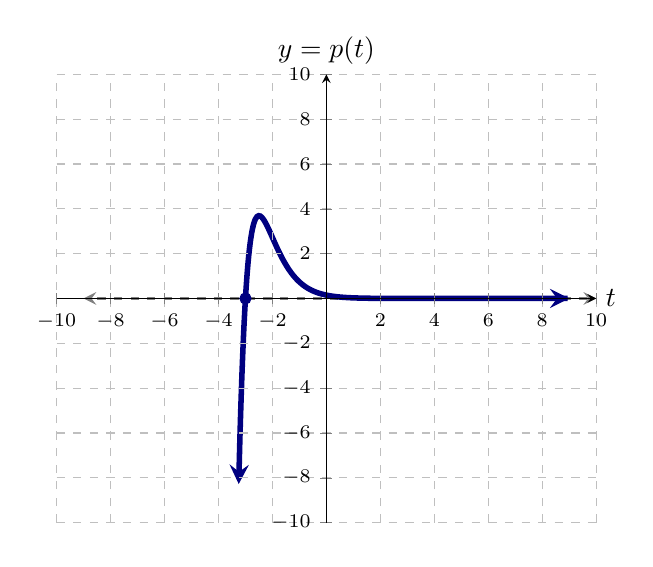
\begin{tikzpicture}
  \begin{axis}[
            domain=-10:10, ymax=10, xmax=10, ymin=-10, xmin=-10,
            axis lines =center, xlabel=$t$, ylabel={$y=p(t)$}, grid = major, grid style={dashed},
            ytick={-10,-8,-6,-4,-2,2,4,6,8,10},
            xtick={-10,-8,-6,-4,-2,2,4,6,8,10},
            yticklabels={$-10$,$-8$,$-6$,$-4$,$-2$,$2$,$4$,$6$,$8$,$10$}, 
            xticklabels={$-10$,$-8$,$-6$,$-4$,$-2$,$2$,$4$,$6$,$8$,$10$},
            ticklabel style={font=\scriptsize},
            every axis y label/.style={at=(current axis.above origin),anchor=south},
            every axis x label/.style={at=(current axis.right of origin),anchor=west},
            axis on top
          ]
          
            \addplot [line width=1, gray, dashed,smooth,samples=200,domain=(-9:10),<->] {0};
            \addplot [line width=2, penColor, smooth,samples=200,domain=(-3.25:9),<->] {(x+3) * e^(-2*x-3)};
            

          %\addplot[color=penColor,fill=penColor2,only marks,mark=*] coordinates{(-6,9)};
          %\addplot[color=penColor,fill=penColor2,only marks,mark=*] coordinates{(2,-7)};

          \addplot[color=penColor,fill=penColor,only marks,mark=*] coordinates{(-3,0)};



           

  \end{axis}
\end{tikzpicture}
\end{image}






\end{example}

































\begin{center}
\textbf{\textcolor{green!50!black}{ooooo-=-=-=-ooOoo-=-=-=-ooooo}} \\

more examples can be found by following this link\\ \link[More Examples of Function Analysis]{https://ximera.osu.edu/csccmathematics/precalculus1/precalculus1/functionAnalysis/examples/exampleList}

\end{center}





\end{document}
